\documentclass[tikz,border=6pt]{standalone}
\usepackage[T1]{fontenc}
\usepackage{lmodern}
\usepackage{amsmath,amssymb}
\usetikzlibrary{arrows.meta,angles,quotes,calc,positioning}
\definecolor{axis}{HTML}{40515F}
\definecolor{grid}{HTML}{DDE4E8}
\definecolor{blue}{HTML}{3568D4}
\definecolor{coral}{HTML}{EF626C}
\definecolor{teal}{HTML}{2A9D8F}
\definecolor{gold}{HTML}{D89432}
\definecolor{purple}{HTML}{7357C8}
\tikzset{
  axisline/.style={axis, line width=.85pt, -{Stealth[length=3mm]}},
  guide/.style={axis!45, line width=.75pt, dashed},
  vector/.style={line width=1.5pt, -{Stealth[length=3mm]}},
  dot/.style={circle, fill=white, draw, line width=1.15pt, inner sep=2.15pt},
  label/.style={font=\large},
  smalllabel/.style={font=\normalsize}
}
\begin{document}

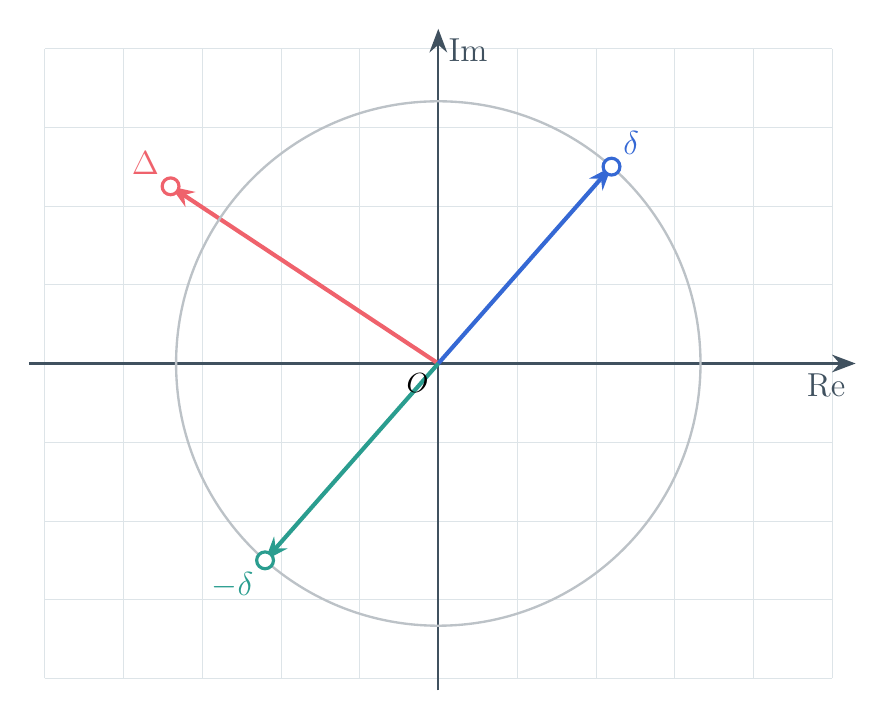
\begin{tikzpicture}[x=1cm,y=1cm]
  \draw[step=1cm,grid,very thin] (-5,-4) grid (5,4);
  \draw[axisline] (-5.2,0)--(5.3,0) node[below left,font=\large] {$\operatorname{Re}$};
  \draw[axisline] (0,-4.15)--(0,4.25) node[below right,font=\large] {$\operatorname{Im}$};
  \coordinate (O) at (0,0);
  \coordinate (D) at (-3.4,2.25);
  \coordinate (R) at (2.2,2.5);
  \coordinate (Rm) at (-2.2,-2.5);
  \draw[coral,line width=1.5pt,-{Stealth[length=3mm]}] (O)--(D);
  \draw[blue,line width=1.5pt,-{Stealth[length=3mm]}] (O)--(R);
  \draw[teal,line width=1.5pt,-{Stealth[length=3mm]}] (O)--(Rm);
  \draw[axis!35,line width=.85pt] (O) circle[radius=3.33];
  \node[dot,draw=coral] at (D) {};
  \node[dot,draw=blue] at (R) {};
  \node[dot,draw=teal] at (Rm) {};
  \node[label,coral,above left=1pt of D] {$\Delta$};
  \node[label,blue,above right=1pt of R] {$\delta$};
  \node[label,teal,below left=1pt of Rm] {$-\delta$};
  \node[smalllabel,below left] at (O) {$O$};
\end{tikzpicture}
\end{document}
